\documentclass[border={10pt 5pt 5pt 5pt},tikz]{standalone}

\usepackage[T1]{fontenc}
\usepackage[sfdefault,scaled=.85]{FiraSans}
\usepackage{tikz}
\usepackage{pgfplots}
\usepackage{ifthen}
\usetikzlibrary{arrows.meta}
\usetikzlibrary{shapes.geometric}
\usetikzlibrary{mindmap,trees,shadows}

\usetikzlibrary{arrows.meta,angles,quotes}
\colorlet{linecol}{black!75}
\usepackage{forest}

\begin{document}

	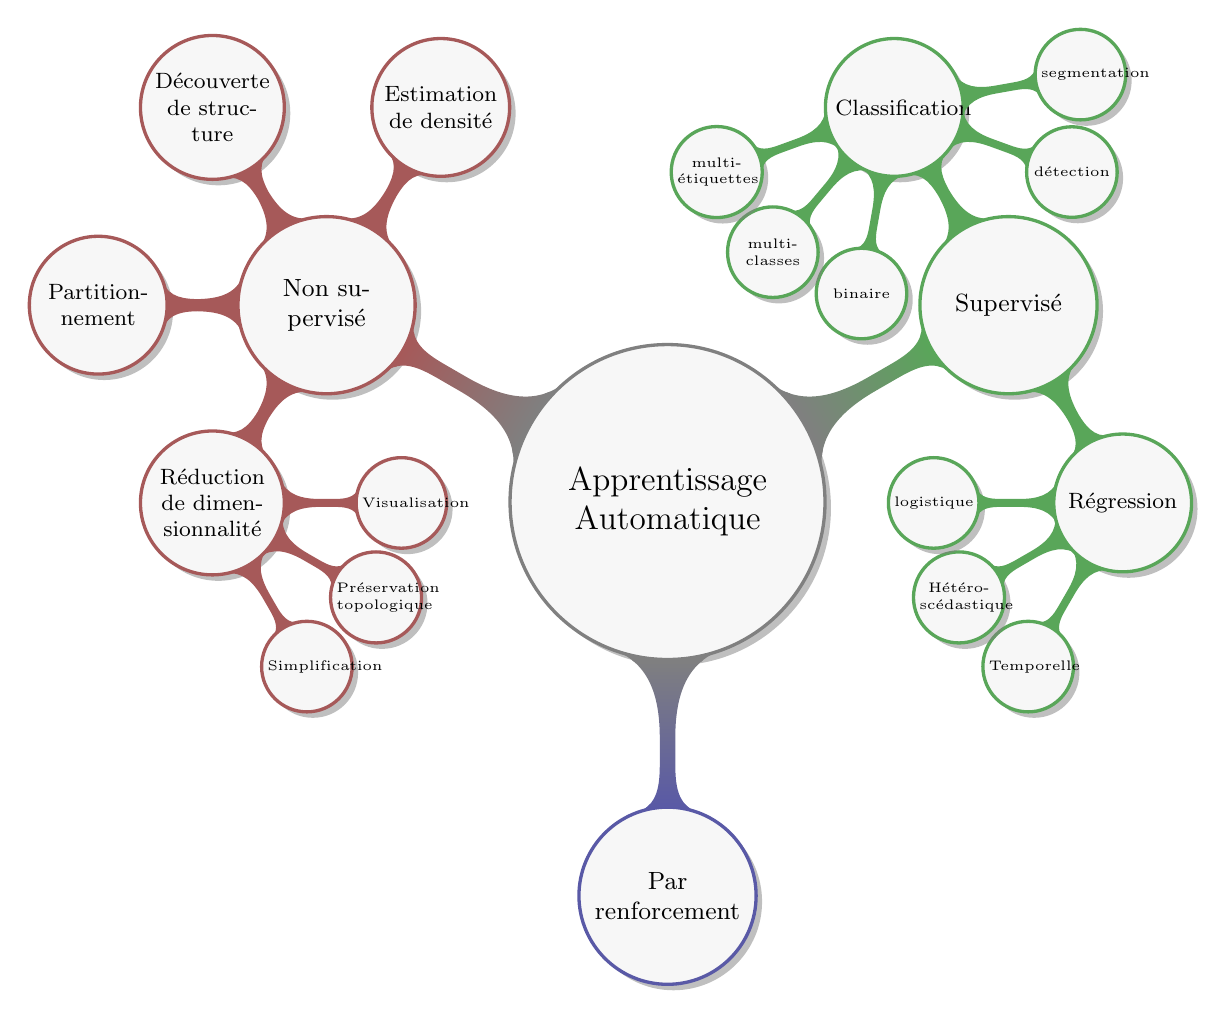
\begin{tikzpicture}
		\tikzset{concept/.append style={fill={black!3},drop shadow}}
		\path[mindmap,concept color=gray,text=black]
		node[concept] {Apprentissage Automatique}
		[clockwise from=30]
		child[concept color=green!30!gray] {
			node[concept] {Supervisé}
			[clockwise from=120]
			child { 
				node[concept] {Classification} 
				[clockwise from=-100]
					child { node[concept] {binaire} }
					child { node[concept] {multi-classes} }
					child { node[concept] {multi-étiquettes} }
					child [clockwise from=70] { node[concept] {détection} }
					child [clockwise from=130] { node[concept] {segmentation} }
			}
			child[sibling angle=180] { 
				node[concept] {Régression} 
				[clockwise from=-120]
					child { node[concept] {Temporelle} }
					child { node[concept] {Hétéro-scédastique} }
					child { node[concept] {logistique} }
			}
		}
		child[concept color=blue!30!gray, sibling angle=120] {
			node[concept] {Par\\renforcement}
			% [clockwise from=0]
			% child { node[concept,font=\footnotesize] {Hors-ligne} }
			% child { node[concept] {} }
			% child { node[concept] {} }
			% child { node[concept] {} }
		}
		child[concept color=red!30!gray, sibling angle=120] {
			node[concept] {Non supervisé}
			[clockwise from=-120]
			child { 
				node[concept] {Réduction de dimensionnalité} 
				[clockwise from=0]
					child { node[concept] {Visualisation} }
					child { node[concept] {Préservation topologique} }
					child { node[concept] {Simplification} }
			}
			child[sibling angle=60] { node[concept] {Partition-nement} }
			child[sibling angle=60] { node[concept] {Découverte de structure} }
			child[sibling angle=60] { node[concept] {Estimation de densité} }
		};
	\end{tikzpicture}

\end{document}
